\documentclass{article}
\usepackage[margin=1in]{geometry}
\usepackage{amsmath}
\usepackage{amssymb}
\usepackage{booktabs}
\usepackage{float}
\usepackage{graphicx}
\usepackage{hyperref}
\usepackage{pdfpages}
\usepackage{siunitx}
\usepackage{adjustbox}
\usepackage{cancel}
\usepackage{paracol}
\usepackage{placeins}

\usepackage{parskip}

\globalcounter{figure}
\counterwithin{equation}{section}

\title{Report}
\date{02 March 2026}
\author{Connor Emmons}

\begin{document}
\pagenumbering{gobble}
\maketitle
\vfill
\paragraph*{Notes}

\newpage
\pagenumbering{arabic}

\section{Initial Tests}

\section{Jacobi and Hamiltonian}

First attempt at plotting Jacobi and Hamiltonian for the chosen best guess at the end of last week. Jacobi looks good, Hamiltonian does not. YAPSS documentation suggests mesh refinement, use Dr. Hall's suggestion of 100, 10.

\begin{figure}[H]
    \centering
    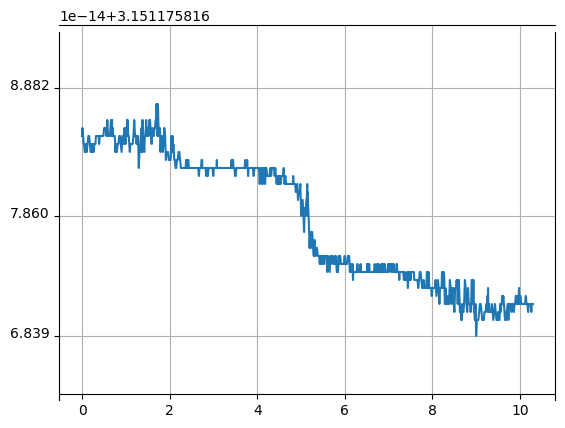
\includegraphics[width=\columnwidth]{jacobi1.png}
    \caption{Jacobi Attempt 1}
    \label{fig: jac-attempt1}
\end{figure}

\begin{figure}[H]
    \centering
    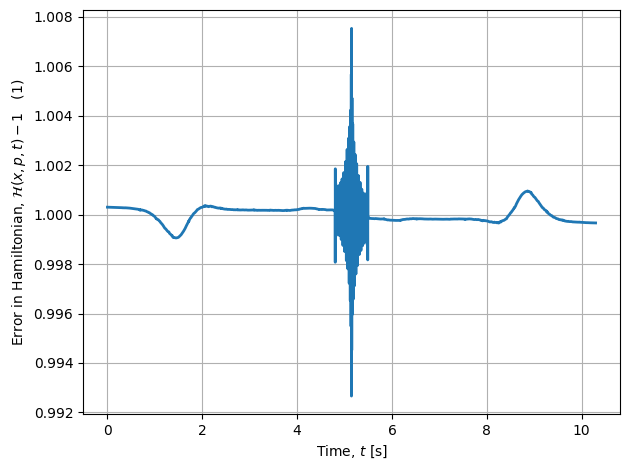
\includegraphics[width=\columnwidth]{hamiltonian1.png}
    \caption{Hamiltonian Attempt 1}
    \label{fig: ham-attempt1}
\end{figure}

Attempt 2 requires no Jacobi or Hamiltonian analysis, the new mesh did not work.

\begin{figure}[H]
    \centering
    
\includegraphics[width=\columnwidth]{attempt2.png}
    \caption{Attempt 2}
    \label{fig: attempt2}
\end{figure}

Next, try guessing the first solution and then resolve using 100, 10 mesh. Jacobi constant got worse (still more than good enough), Hamiltonian stayed the same, but at least the shapes match.

Note: All further Jacobi graphs with 0 at the midpoint of the y-axis are plotting the difference between the Jacobi constant and the mean of the Jacobi constant across all steps.

\begin{figure}[H]
    \centering
    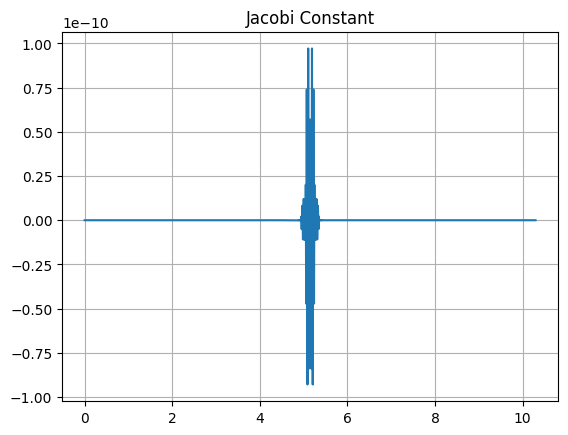
\includegraphics[width=\columnwidth]{jacobi2.png}
    \caption{Jacobi Attempt 2}
    \label{fig: jac-attempt2}
\end{figure}

\begin{figure}[H]
    \centering
    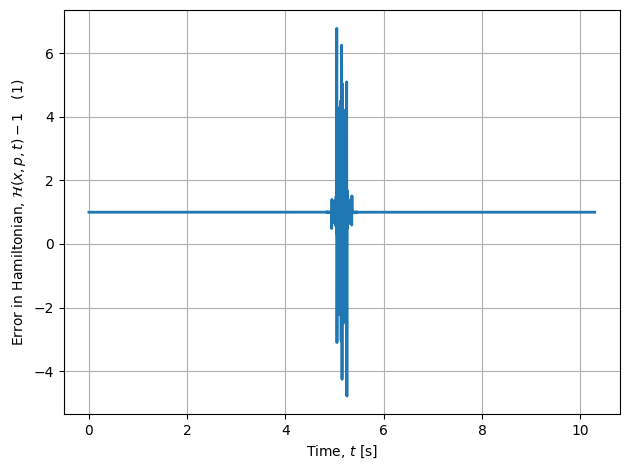
\includegraphics[width=\columnwidth]{hamiltonian2.png}
    \caption{Hamiltonian Attempt 2}
    \label{fig: ham-attempt2}
\end{figure}

Resetting the final time bounds for the second solution off of the first solution as a guess to 0 and infinity gives a orbit with a period that is 1.7\% off of what was stated in the paper ($\sim$18 hours), but the Jacobi and Hamiltonian match and the Hamiltonian is much closer to 1.

\begin{figure}[H]
    \centering
    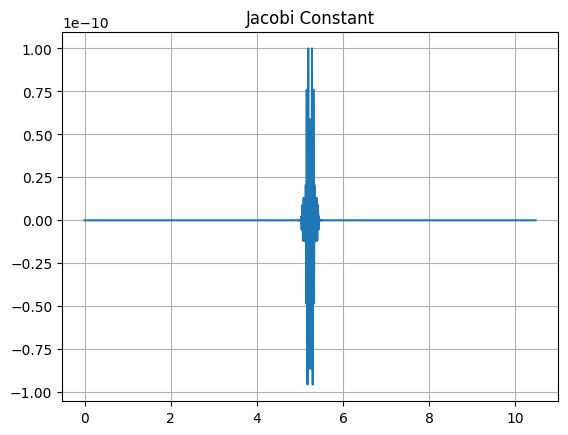
\includegraphics[width=\columnwidth]{jacobi3.png}
    \caption{Jacobi Attempt 3}
    \label{fig: jac-attempt3}
\end{figure}

\begin{figure}[H]
    \centering
    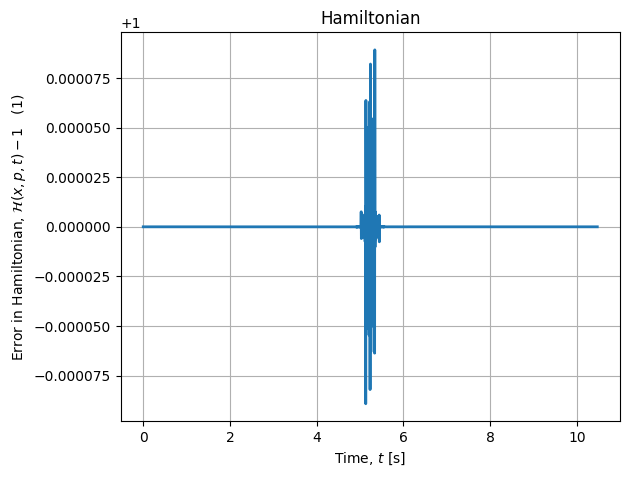
\includegraphics[width=\columnwidth]{hamiltonian3.png}
    \caption{Hamiltonian Attempt 3}
    \label{fig: ham-attempt3}
\end{figure}

Changing the ipopt tolerance to 1e-16 from 1e-100 was not a productive change.

\begin{figure}[H]
    \centering
    
\includegraphics[width=\columnwidth]{attempt4.png}
    \caption{Attempt 4}
    \label{fig: attempt4}
\end{figure}

Changing back to a tolerance of 1e-100 and splitting the two solutions into their own code blocks shows that the first solution takes $\sim$20 seconds, and the second takes $\sim$5 seconds.

\section{One Solution with New Bounds and Mesh}

Removing the bounds on the final time and only solving once, but with a mesh of 100, 10, yields interesting results (but not a useful orbit).

\begin{figure}[H]
    \centering
    
\includegraphics[width=\columnwidth]{attempt5.png}
    \caption{Attempt 5}
    \label{fig: attempt5}
\end{figure}

\begin{figure}[H]
    \centering
    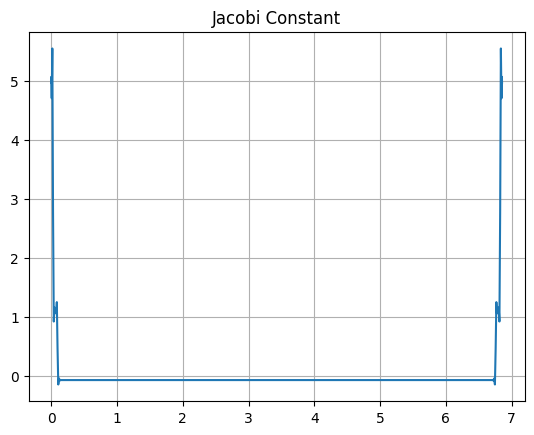
\includegraphics[width=\columnwidth]{jacobi5.png}
    \caption{Jacobi Attempt 5}
    \label{fig: jac-attempt5}
\end{figure}

\begin{figure}[H]
    \centering
    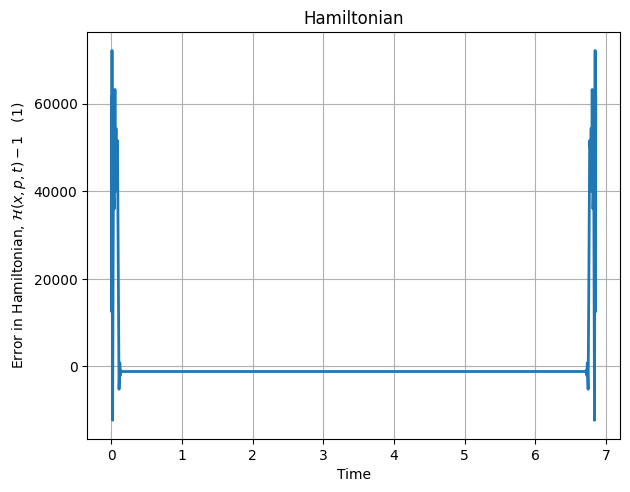
\includegraphics[width=\columnwidth]{hamiltonian5.png}
    \caption{Hamiltonian Attempt 5}
    \label{fig: ham-attempt5}
\end{figure}

Kept the loose bounds, but increased the number of segments to 150. Interestingly, YAPSS found a solution which conserves the Jacobi constant, but the Jacobi constant is incorrect (2.9723050606473316 vs 3.151175879508174). The Hamiltonian exhibits the same small deviation, but is also offset. Also, the run time of this solution was significantly shorter than expected, indicating that if the Jacobi constant deviation/Hamiltonian deviation is low (i.e., YAPSS converged on a solution), then the run should't take long.

\begin{figure}[H]
    \centering
    
\includegraphics[width=\columnwidth]{attempt7.png}
    \caption{Attempt 7}
    \label{fig: attempt7}
\end{figure}

\begin{figure}[H]
    \centering
    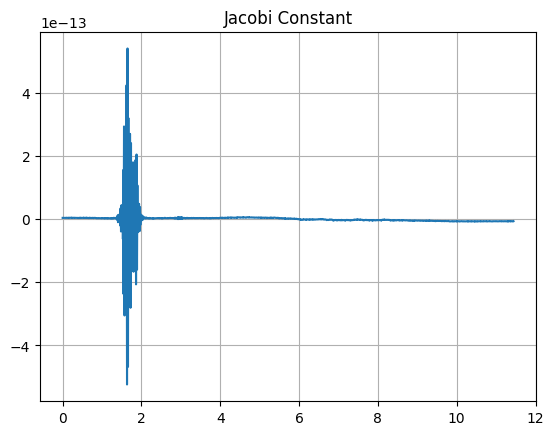
\includegraphics[width=\columnwidth]{jacobi7.png}
    \caption{Jacobi Attempt 7}
    \label{fig: jac-attempt7}
\end{figure}

\begin{figure}[H]
    \centering
    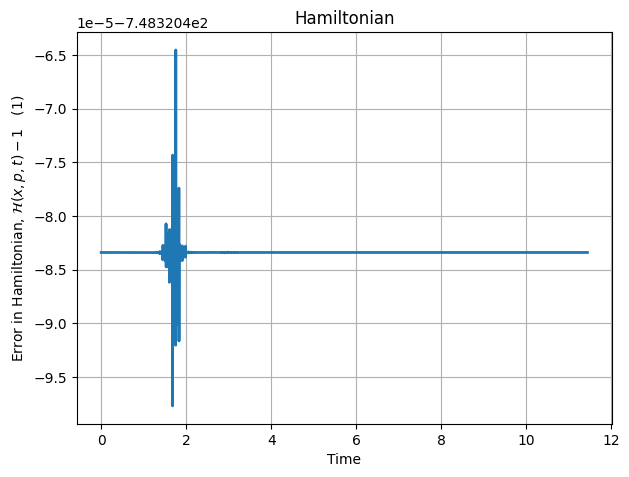
\includegraphics[width=\columnwidth]{hamiltonian7.png}
    \caption{Hamiltonian Attempt 7}
    \label{fig: ham-attempt7}
\end{figure}

Increase segments to 200. Jacobi constant incorrect but close (3.134456975968208 vs 3.151175879508174); reflected in Hamiltonian somewhat (better with better scaling).

\begin{figure}[H]
    \centering
    
\includegraphics[width=\columnwidth]{attempt8.png}
    \caption{Attempt 8}
    \label{fig: attempt8}
\end{figure}

\begin{figure}[H]
    \centering
    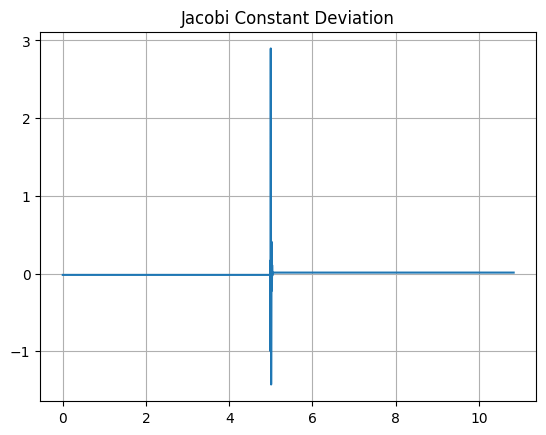
\includegraphics[width=\columnwidth]{jacobi8.png}
    \caption{Jacobi Attempt 8}
    \label{fig: jac-attempt8}
\end{figure}

\begin{figure}[H]
    \centering
    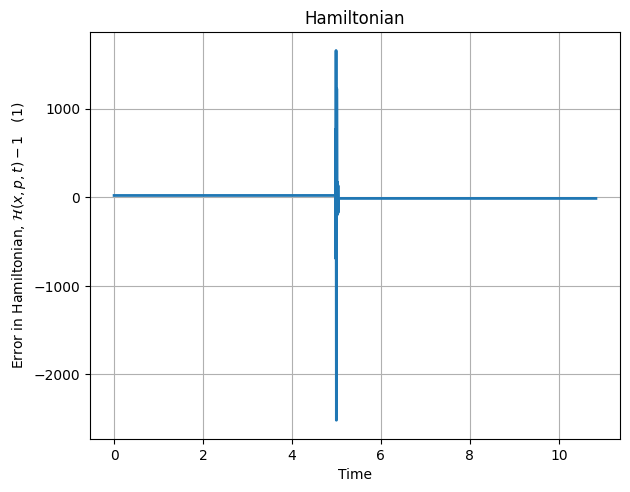
\includegraphics[width=\columnwidth]{hamiltonian8.png}
    \caption{Hamiltonian Attempt 8}
    \label{fig: ham-attempt8}
\end{figure}

\section{First 3D Attempts}

While this solution looks very similar to the good 2D solution, it is different. For this one, the period is 10.1628 vs 10.47 for the good orbit (this gives 1.26\% error with the number provided in the paper). While the Jacobi constant is almost identitical to the good 2D solution, the Hamiltonian is way off. Notably, the second solution (that used the first solution as an initial guess) took considerably longer to run (over 1 minute).

\begin{figure}[H]
    \centering
    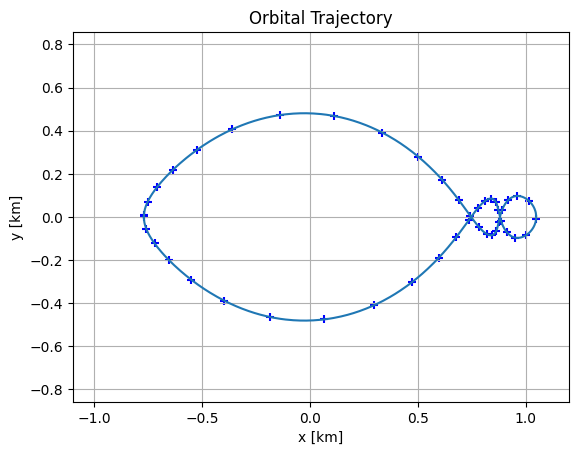
\includegraphics[width=\columnwidth]{3Dattempt1.png}
    \caption{3D Attempt 1}
    \label{fig: 3Dattempt1}
\end{figure}

\begin{figure}[H]
    \centering
    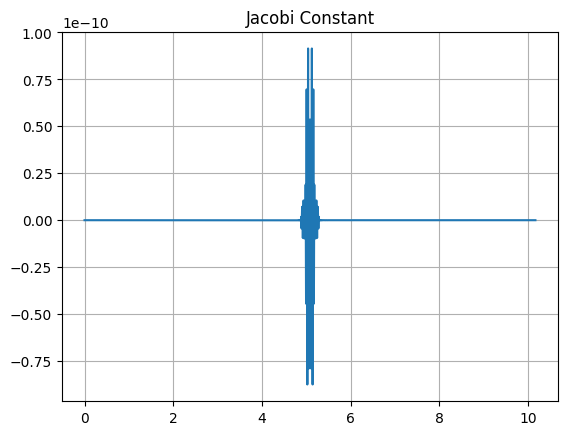
\includegraphics[width=\columnwidth]{3Djacobi1.png}
    \caption{3D Jacobi Attempt 1}
    \label{fig: 3Djac-attempt1}
\end{figure}

\begin{figure}[H]
    \centering
    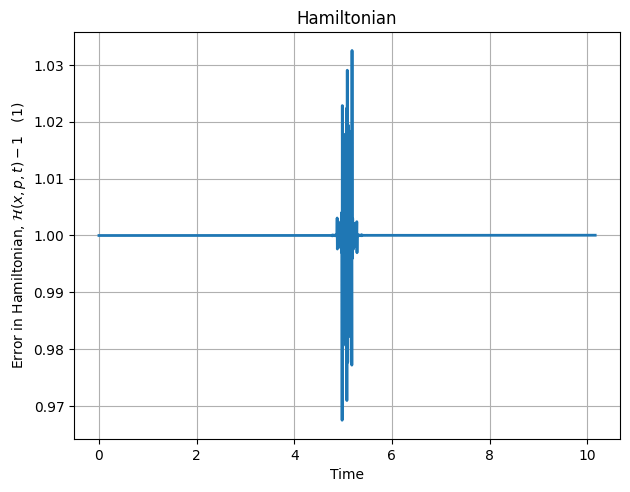
\includegraphics[width=\columnwidth]{3Dhamiltonian1.png}
    \caption{3D Hamiltonian Attempt 1}
    \label{fig: 3Dham-attempt1}
\end{figure}

Shown below is the first solution. Note that the Jacobi constant is quite good, but the Hamiltonian is poor.

\begin{figure}[H]
    \centering
    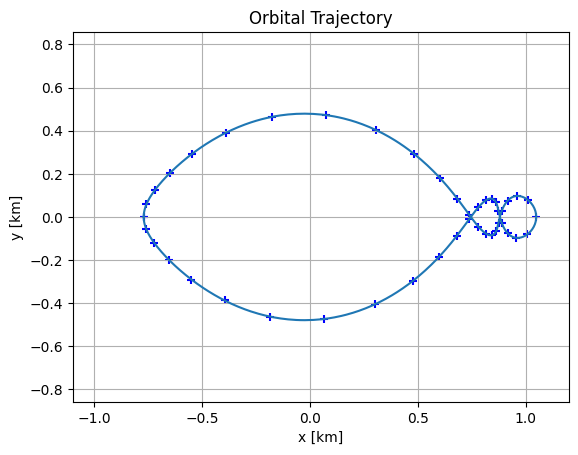
\includegraphics[width=\columnwidth]{3Dfirstguess.png}
    \caption{3D First Guess}
    \label{fig: 3Dfirstguess}
\end{figure}

\begin{figure}[H]
    \centering
    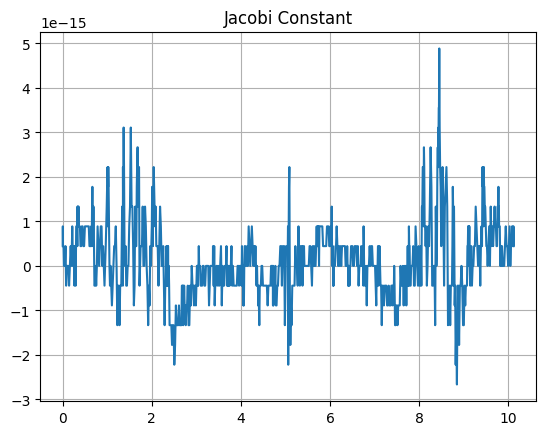
\includegraphics[width=\columnwidth]{3Dfirstguessjacobi.png}
    \caption{3D First Guess Jacobi}
    \label{fig: 3Djac-firstguess}
\end{figure}

\begin{figure}[H]
    \centering
    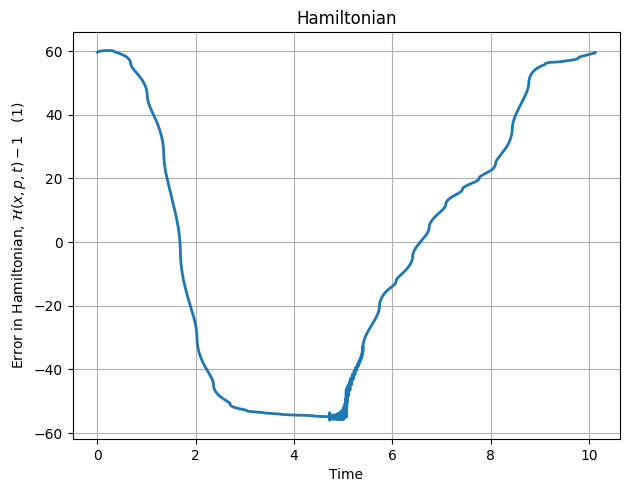
\includegraphics[width=\columnwidth]{3Dfirstguesshamiltonian.png}
    \caption{3D First Guess Hamiltonian}
    \label{fig: 3Dham-firstguess}
\end{figure}

\end{document}